\chapter{课外实验活动}

\section{自制指南针}
如图~\ref{fig_C_10-10} 所示,用硬纸板、大头针、按扣、缝衣针自制一
个指南针.

用磁铁的一端在缝衣针上
朝一个方向擦几下,缝衣针就
有了磁性.为了使缝衣针能顺
利地穿过按扣(取按扣中较薄
的一扇)的两个小孔,可用钳子
把按扣的边缘向下夹一下.
当自制的指南针静下来后,记住针的哪一端指北.

\begin{figure}[htbp]
    \centering
    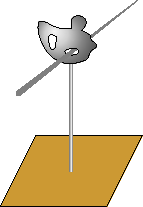
\includegraphics{fig/C/10-10.pdf}
    \caption{}\label{fig_C_10-10}
\end{figure}


\section{验证环形电流的磁场}
这个实验是用自制的指南针来验证环形电流的磁场方向
(图~\ref{fig_C_10-11}).
在一个瓶子(或硬纸筒)上用漆包线绕一个10至15
匝的线圈,把绕好的线圈从瓶子上取下来,再用胶布把线圈竖
直固定在一块木板上.
将你自制的指南针放在图~\ref{fig_C_10-11} 所示
的位置,转动木板使磁针处在线圈平面内.
用学过的环形电
流磁场的知识判断一下,如果线圈的两端接上电池,指南针将
怎样偏转.
然后再给线圈通电,看一看实验结果跟你的判断
是否一致.
\begin{figure}[htbp]
    \centering
    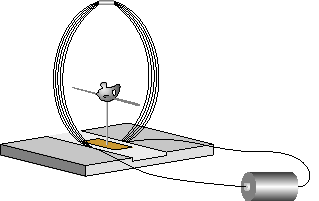
\includegraphics{fig/C/10-11.pdf}
    \caption{}\label{fig_C_10-11}
\end{figure}

    \section{验证通电螺线管的南北极}
把漆包线绕在一支铅笔上,然后抽出铅笔,做成一个螺线
管.用学过的通电螺线管磁场的知识判断一下,如果给螺线
管通电,通电螺线管哪端是南极,哪端是北极.然后把自制的
指南针放在螺线管的两端,给螺线管通电,看看实验结果跟你
的判断是否一致.

\section{观察磁化现象}
取一个条形磁铁和一个大铁钉.
把铁钉插入铁屑,并把
条形磁铁的一个磁极靠近钉子头.
然后同时提起磁铁和铁钉,
你将看到一些铁屑粘到钉子上.将磁铁移去,铁钉上的大部
分铁屑将掉下来,但仍有一部分铁屑粘在钉子上.再用磁铁
的另一个磁极靠近钉子头,剩在钉子上的铁屑就会掉下来.

解释上述现象.

\section{判断指南针的偏转方向}
在一个铅笔刀或一个大些的铁钉上,用漆包线绕上两个
线圈$A$和$B$,将线圈$B$的两端接在一起,并把$CD$段漆包线放
在静止的自制指南针的上方(图~\ref{fig_C_10-12}).试判断当用干电池
给线圈$A$通电的一瞬间,指南针偏转的方向.做这个实验,看
一看你判断的指南针偏转方向与实验是否一致.
\begin{figure}[htbp]
    \centering
    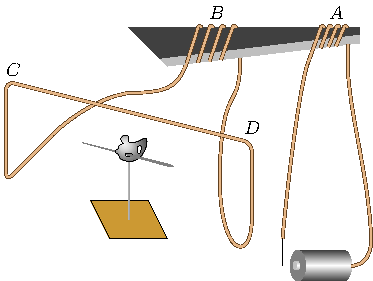
\includegraphics{fig/C/10-12.pdf}
    \caption{}\label{fig_C_10-12}
\end{figure}

\section{自制测电笔}
准备一个小氖灯,一个小弹簧.
再找一个装中药片的小
玻璃瓶,两个瓶盖,两个铁钉,一个$0.25$瓦、$2 \sim 5$兆欧的电阻.
在稍粗糙的水泥砖上把玻璃瓶底磨掉,做成一个玻璃圆筒.
让铁钉穿过瓶盖,盖上瓶盖后使钉帽在瓶里.
把电阻的两根引
线齐根去掉,并把电阻两端的绝缘漆去掉.照图~\ref{fig_C_10-13} 那样
把上述器材安装起来,就做成了一个测电笔.
\begin{figure}[htbp]
    \centering
    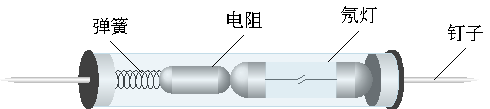
\includegraphics{fig/C/10-13.pdf}
    \caption{自制测电笔}\label{fig_C_10-13}
\end{figure}

用这个自制的测电笔可以辨别照明电路的火线和地线.
用拇指和食指拿住玻璃瓶,前面的钉子接触待辨别的导线,后
面的钉子接触手.当前面的钉子接触的是火线时,小氖灯发
光;接触的是地线时,小氖灯不发光.这样就可以辨别出火线
和地线.

要注意:\NoteUnderWave{手的任何部位都不要接触前面的钉子},因为它
接触的可能是火线,会使人触电.

\section{测定水的折射率}
找一个广口瓶,在瓶内盛
满水,照图~\ref{fig_C_10-14} 那样把直尺$AB$
紧挨着瓶口的$C$点竖直插入瓶内.
从尺的对面一点$P$观察水
面,可以同时看到直尺在水中
的部分和露出水面的部分在水
中的像.读出你看到的直尺水
下部分最低点的刻度$S_1$,以及
跟这个刻度相重合的、水上部
分刻度$S_2$的像$S'_2$.记下$CS_1$和
$CS_2$的长度,量出广口瓶瓶口的内径$d$,就能算出水的折射率.
你用这种方法求出的水的折射率为多少?
\begin{figure}[htbp]
	\centering
	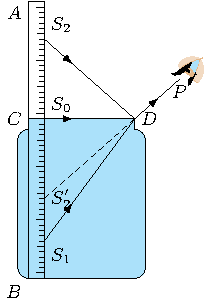
\includegraphics{fig/C/10-14.pdf}
	\caption{}\label{fig_C_10-14}
\end{figure} 

 
如果你能同时读出直尺在水下的两个刻度$S_1$和$S_3$,以
及跟它们相重合的、两个水上刻度$S_2$和$S_4$在水中的像$S'_2$和
$S'_4$,就可以不必测量瓶口的内径,直接用从直尺上读出的两
组数据求出水的折射率来.比较这两种方法测量的结果,看
哪种方法测得的折射率更准确?

用后一种方法进行测量,瓶中的水不一定非盛满不可,竖
直插入水中的直尺也不一定要紧挨瓶口,做起来更简便.

\section{测定凹透镜的焦距}
凹透镜所成的虚像不能在像屏上显示出来,因此它的焦
距不可能像凸透镜那样直接利用焦点或成像方法来测量.
下面介绍一种测量凹透镜焦距的简便方法.

\begin{figure}[htbp]
	\centering
	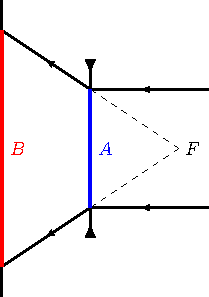
\includegraphics{fig/C/10-15.pdf}
	\caption{}\label{fig_C_10-15}
\end{figure}


在凹透镜的中心贴一个半径为$R$的黑色圆纸片$A$,另取
一张白纸$B$,在$B$上画一个半径为$2R$的圆.把白纸和凹透镜
平行地放在太阳光下(图~\ref{fig_C_10-15}),让透镜对着太阳,调节透镜
和白纸间的距离,使黑色圆纸片的影恰好跟白纸上的圆圈重
合.这时透镜和白纸间的距离就等于凹透镜的焦距.想想看,
为什么?做这个实验,并将测得的焦距跟已知的焦距相比较,
看相差多少.




